\documentclass[10pt,xcolor=table]{beamer}

\usetheme{metropolis}
\usepackage{appendixnumberbeamer}

\usepackage{booktabs}
\usepackage[scale=2]{ccicons}

\usepackage{multirow}
% \usepackage{multicolumn}

\usepackage{pgfplots}
\usepgfplotslibrary{dateplot}

\usepackage{xspace}
\newcommand{\themename}{\textbf{\textsc{metropolis}}\xspace}

\title{Optimasi Pencocokan Pola dalam Sistem Deteksi Intrusi Snort Menggunakan GPU}
% \subtitle{A modern beamer theme}
\date{}
\author{Afrizal Fikri}
\institute{13513004}
% \titlegraphic{\hfill\includegraphics[height=1.5cm]{logo.pdf}}

\makeatletter
\def\Ldescription{%
  \@ifnextchar[{\beamer@testforospec}{\beamer@descdefault\beamer@descriptionwidth\@@Ldescription}%
}

\def\beamer@testforospec[{\@ifnextchar<{\beamer@scandefaultospec[}{\@Ldescription[}}%

\def\beamer@scandefaultospec[#1]{\def\beamer@defaultospec{#1}\Ldescription}

\def\@Ldescription[#1]{%
\setbox\beamer@tempbox=\hbox{\def\insertdescriptionitem{#1}
  \usebeamertemplate**{description item}}%
\beamer@descdefault\wd\beamer@tempbox\@@description%
}%

\def\@@Ldescription{%
  \beamer@descdefault35pt%
  \list
  {}
  {\labelwidth\beamer@descdefault\leftmargin2.8em\let\makelabel\beamer@Ldescriptionitem}%
  \beamer@cramped%
  \raggedright
  \beamer@firstlineitemizeunskip%
}

\def\endLdescription{\ifhmode\unskip\fi\endlist}
\long\def\beamer@Ldescriptionitem#1{%
  \def\insertdescriptionitem{#1}%
  \hspace\labelsep{\parbox[b]{\dimexpr\textwidth-\labelsep\relax}{%
        \usebeamertemplate**{description item}%
    }}}
\makeatother

\begin{document}

\maketitle

\begin{frame}{Overview}
    \setbeamertemplate{section in toc}[sections numbered]
    \tableofcontents[hideallsubsections]
\end{frame}

\section{Permasalahan}

\begin{frame}[fragile]{Definisi}
    \begin{Ldescription}

        \item[Intrusi] Serangkaian percobaan yang tidak berhak baik bertujuan untuk merusak maupun tidak terhadap sumber daya

        \item[Sistem deteksi intrusi] Mekanisme yang mengotomasi proses deteksi dan pencegahan intrusi terhadap satu atau beberapa sumber daya

        \item[\emph{Signature}] Pola tertentu yang terdapat pada paket seperti \emph{byte payload} atau servis tertentu

    \end{Ldescription}
\end{frame}

\begin{frame}[fragile]{Sistem Deteksi Intrusi}

    Beberapa metode deteksi intrusi:
    \begin{enumerate}
        
        \item \emph{Signature-based detection} \\
        Pencocokan dilakukan berdasarkan \emph{signature} yang telah disiapkan
        
        \item \emph{Anomaly-based detection} \\
        Pencocokan dilakukan dengan membandingkan profil dengan \emph{threshold} tertentu
        
        \item \emph{Stateful protocol analysis} \\
        Pencocokan dilakukan secara dalam dengan melihat rangkaian protokol dalam \emph{traffic}
    
    \end{enumerate}    
\end{frame}

\begin{frame}[fragile]{Latar Belakang}
    \begin{itemize}

        \item Peningkatan kapasitas \emph{traffic} jaringan dan jenis serangan

        \item Diperlukan sumber daya besar untuk analisis \emph{traffic} jaringan

        \item Porsi analisis terbesar ada pada bagian pencocokan string

        \item Perkembangan GPU yang lebih cepat dan murah sebagai alternatif penggunaan CPU
        \item Kebutuhan akan implementasi pada GPU yang meminimalkan latensi

    \end{itemize}
\end{frame}

\begin{frame}[fragile]{Rumusan Masalah}
    \begin{enumerate}

        \item Bagaimana implementasi pencocokan pola dengan GPU pada IDS Snort?

        \item Bagaimana kinerja sistem deteksi intrusi jaringan akibat dari penggunaan GPU?

    \end{enumerate}
\end{frame}

\begin{frame}[fragile]{Tujuan}
    \begin{enumerate}
        
        \item Mengembangkan modul pencocokan pola dengan GPU yang terintegrasi dengan Snort IDS
        
        \item Melakukan perbandingan kinerja sistem deteksi intrusi jaringan sebelum dan setelah menggunakan GPU

    \end{enumerate}
\end{frame}

\section{Analisis}

\begin{frame}{Analisis}
    \begin{itemize}

        \item Algoritma pencocokan \emph{signature}

        \item Struktur penyimpanan kamus

        \item Alokasi \emph{thread}

        \item Optimasi latensi pada GPU

    \end{itemize}
\end{frame}

\begin{frame}[fragile]{Algoritma Pencocokan String}
    \begin{itemize}

        \item Pencocokan string menurut sumbernya ada 2 macam: \emph{single pattern} dan \emph{multi pattern}

        \item Pada \emph{multi pattern string matching}, pola akan dikumpulkan dalam sebuah kamus
    
        \item Pencocokan dilakukan dengan pembacaan dari kamus sekaligus

    \end{itemize}
\end{frame}

\begin{frame}{Algoritma Pencocokan \emph{Signature}}
    \begin{figure}
        \centering
        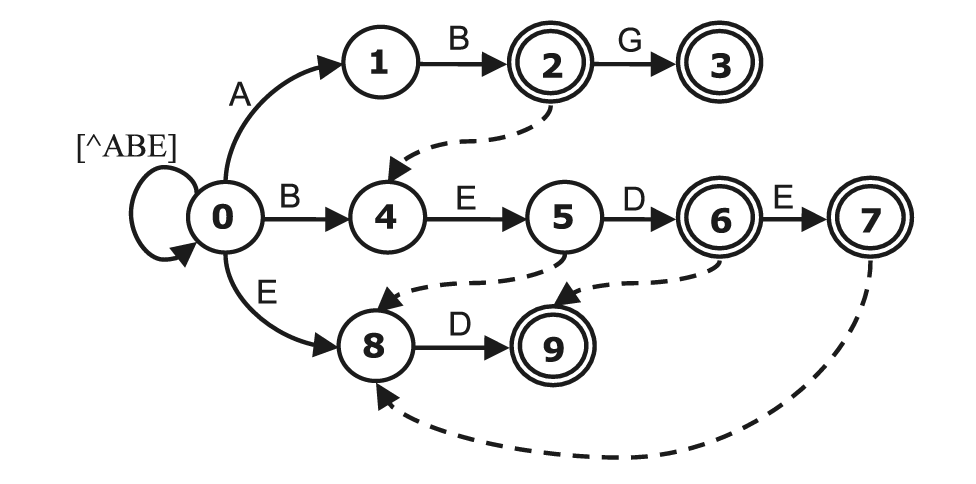
\includegraphics[width=0.5\textwidth]{../src/resources/aho-c.png}
    \end{figure}

    Algoritma akan dikembangkan dengan berbasis algoritma Aho-Corasick karena:
    \begin{itemize}
        \item mampu melakukan pencocokan kamus dalam sekali penelusuran
        \item stabil terhadap jumlah 
        \item memiliki kinerja paling baik pada IDS Snort
    \end{itemize}
\end{frame}

\begin{frame}{Algoritma Pencocokan \emph{Signature}}
    Adaptasi Aho-Corasick untuk memaksimalkan pencocokan secara \emph{multithreading}:
    \begin{columns}[T,onlytextwidth]
        \column{0.5\textwidth}

            \begin{block}{\emph{Data Parallel} AC}
                \emph{Stream input} di partisi menjadi beberapa bagian, kemudian masing-masing akan dilakukan pencocokan dengan satu \emph{thread}
            \end{block}

            \begin{figure}
                \centering
                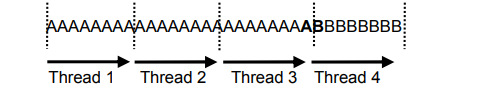
\includegraphics[width=1.0\textwidth]{../src/resources/boundary.png}
            \end{figure}
    
        \column{0.5\textwidth}
    
            \begin{block}{\emph{Parallel Failureless} AC}
                Masing-masing \emph{thread} akan memulai pencocokan dari satu karakter dari \emph{stream input} untuk mencari satu pola
            \end{block}
    
            \begin{figure}
                \centering
                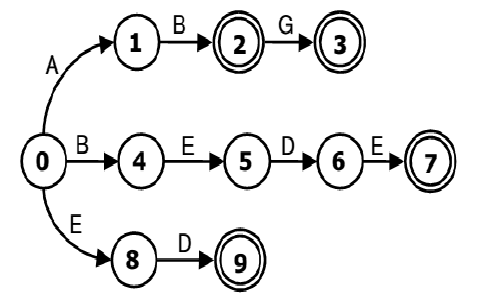
\includegraphics[width=0.7\textwidth]{../src/resources/pfac.png}
            \end{figure}

    \end{columns}
\end{frame}

\begin{frame}{Algoritma Pencocokan \emph{Signature}}
    \begin{table}
    \begin{tabular}{@{} p{5cm}p{5cm} @{}}
        \toprule
        DPAC & PFAC\\
        \midrule
        Porsi tiap \emph{thread seimbang} & \emph{Thread} memiliki umur yang pendek \\
        Butuh ekstensi sepanjang pola terpanjang minus satu & Tiap \emph{thread} hanya bertugas mencari satu pola\\
            & Banyak terjadi \emph{overlap} dalam akses \emph{stream input}\\
        % \emph{Matcher kernel} & Kode GPU yang melakukan penelusuran \emph{state machine}\\
        % \emph{Reducer} & Komponen yang menggabungkan hasil pencocokan untuk dikembalikan ke Snort\\
        \bottomrule
    \end{tabular}
    \end{table}
\end{frame}

\begin{frame}[fragile]{Struktur Penyimpanan Kamus}
    \begin{itemize}

        \item Pola akan disusun dalam struktur tertentu, seperti \emph{tabel} atau \emph{linked trie}
        
        \item Struktur data menentukan operasi pencocokan

        \item \emph{Spatial locality} dapat berpengaruh pada keseluruhan latensi sistem

    \end{itemize}
\end{frame}

\begin{frame}{Struktur Penyimpanan Kamus}
    Pendekatan representasi \emph{state machine}:
    \begin{columns}[T,onlytextwidth]
        \column{0.5\textwidth}

            \begin{block}{\emph{Linked trie}}
            \begin{itemize}
                \item Status terenkapsulasi
                \item Mudah dimodifikasi
            \end{itemize}
            \end{block}
    
        \column{0.5\textwidth}
    
            \begin{block}{Tabel transisi}
            \begin{itemize}
                \item Mudah diimplementasi
                \item Cenderung statik
            \end{itemize}
            \end{block}
    
    \end{columns}
\end{frame}

\begin{frame}{Alokasi \emph{Thread}}
    \begin{itemize}

        \item \emph{Thread} PFAC akan banyak yang berhenti sangat awal

        \item Kinerja \emph{warp} menjadi tidak seimbang

        \item Dapat diatasi dengan skema \emph{assignment} berulang

    \end{itemize}
\end{frame}

\begin{frame}{Optimasi Latensi pada GPU}
    \begin{itemize}

        \item Mengurangi transaksi ke memori global
        \begin{itemize}
            \item Memuat masukan dari memori global ke \emph{shared memory} dengan memanfaatkan \emph{coalescing}
            \item Membaca masukan yang \emph{overlap} cukup dari \emph{shared memory}
        \end{itemize}

        \item Mengurangi latensi ke tabel transisi
        \begin{itemize}
            \item Mengikat tabel transisi ke memori tekstur
            \item Memuat baris pertama ke \emph{shared memory}
        \end{itemize}

        \item Mengurangi \emph{swappiness} pada \emph{input buffer} dengan \emph{pinned memory}

    \end{itemize}
\end{frame}

\section{Rancangan dan Implementasi}

\begin{frame}{Rancangan Solusi}
    
    Pencocokan akan menggunakan implementasi PFAC dengan optimasi dengan memori tekstur dan \emph{pinned memory}

    Secara umum, ada 3 tahap yang akan dilakukan oleh modul yang dikembangkan:
    \begin{enumerate}
        
        \item Pembentukan tabel transisi
        
        \item Pemuatan tabel transisi dalam \emph{device memory}
        
        \item Penelusuran otomata

    \end{enumerate}
\end{frame}

\begin{frame}{Tabel Transisi}
    \begin{figure}
        \centering
        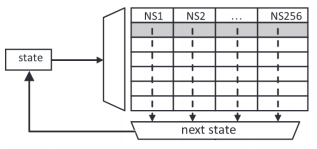
\includegraphics[width=1.0\textwidth]{../src/resources/table.png}
    \end{figure}
\end{frame}

\begin{frame}{Arsitektur Snort}
    \begin{figure}
        \centering
        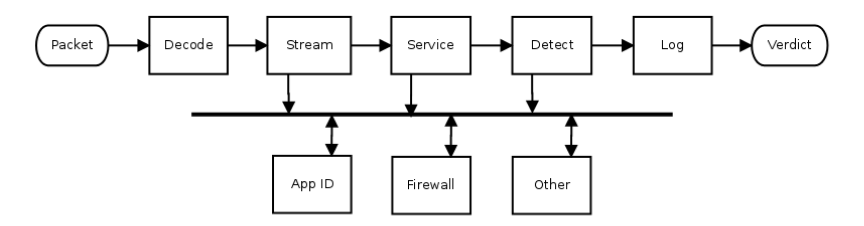
\includegraphics[width=1.0\textwidth]{../src/resources/snort3.png}
    \end{figure}
\end{frame}

\begin{frame}{Arsitektur Modul}
    \begin{figure}
        \centering
        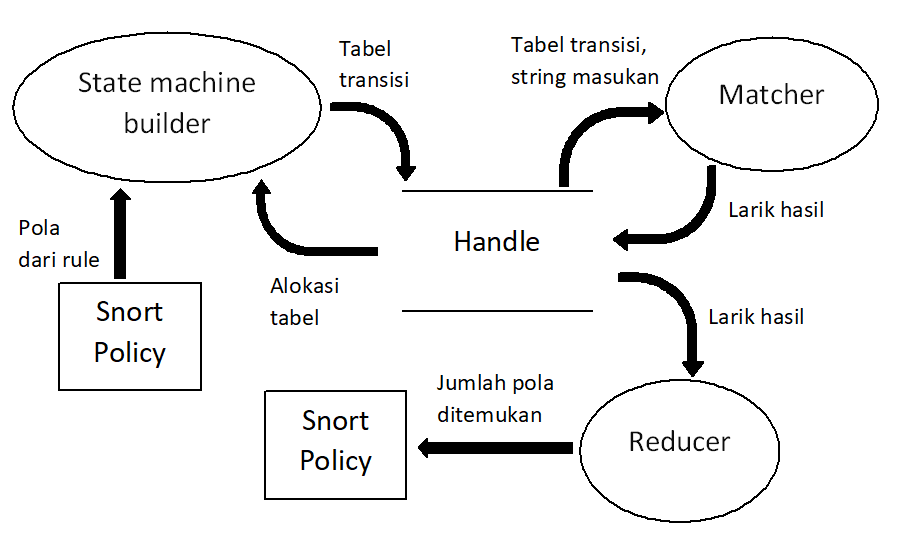
\includegraphics[width=0.6\textwidth]{../src/resources/module-arch.png}
    \end{figure}
\end{frame}

\begin{frame}{Spesifikasi Komponen}
    \begin{table}
    \begin{tabular}{@{} llp{7cm} @{}}
        \toprule
        No & Komponen & Spesifikasi\\
        \midrule
        1. & \emph{Handle} & Struktur data yang membungkus fungsionalitas pencocokan untuk memanggil komponen terkait\\
        2. & \emph{State machine} & Kamus yang digunakan dalam pencocokan\\
        3. & \emph{Kernel wrapper} & \emph{Wrapper} yang menyiapkan \emph{payload} sebelum kode \emph{kernel} dijalankan\\
        4. & \emph{Matcher kernel} & Kode GPU yang melakukan penelusuran \emph{state machine}\\
        5. & \emph{Reducer} & Komponen yang menggabungkan hasil pencocokan untuk dikembalikan ke Snort\\
        \bottomrule
    \end{tabular}
    \end{table}
\end{frame}

\section{Pengujian}

\begin{frame}{Skenario Pengujian}
    Pengujian dilakukan dengan melakukan analisis paket dalam berkas PCAP. Berkas didapatkan dari arsip DEFCON sebesar 2,6 GB

    Pengujian dilakukan dengan besar \emph{buffer} berbeda dan 5 skenario:
    \begin{enumerate}
        \item \emph{Baseline} (AC \emph{multithread} CPU)
        \item Skenario 1: PFAC dengan \emph{global memory}
        \item Skenario 2: PFAC dengan \emph{shared memory}
        \item Skenario 3: PFAC dengan \emph{shared memory} dan \emph{pinned memory}
        \item Skenario 4: PFAC dengan \emph{shared memory}, \emph{pinned memory} dan \emph{texture memory}
    \end{enumerate}
\end{frame}

\begin{frame}{Hasil Pengujian}
    \begin {table}[h]
        \begin{center}
            \resizebox{\textwidth}{!}{%
            \begin{tabular}{ccccccccccc}

            \hline
            % \rowcolor{gray!10}
            \multirow{2}{*}{\emph{Buffer} (kB)} & \emph{Baseline} & \multicolumn{2}{c}{Skenario 1} & \multicolumn{2}{c}{Skenario 2} \\
            \cline{2-6}
            % \rowcolor{gray!10}
            & \emph{Runtime} (detik) & \emph{Runtime} (detik) & \emph{Speedup} & \emph{Runtime} (detik) & \emph{Speedup} \\
            \hline

            128 & 94.632 & 450.629 & 0.21 & 29.207 & 3.4 \\

            512 & 92.656 & 463.281 & 0.2 & 39.321 & 3.16 \\

            1024 & 90.118 & 500.656 & 0.18 & 31.29 & 2.88 \\

            2048 & 96.097 & 436.805 & 0.22 & 31.302 & 3.07 \\
            \hline

            \end{tabular}}
        \end{center}
    \end{table}
\end{frame}

\begin{frame}{Hasil Pengujian (bagian 2)}
    \begin {table}[h]   
        \begin{center}
            \resizebox{\textwidth}{!}{%
            \begin{tabular}{ccccccccccc}

            \hline
            % \rowcolor{gray!10}
            \multirow{2}{*}{\emph{Buffer} (kB)} & \emph{Baseline} & \multicolumn{2}{c}{Skenario 3} & \multicolumn{2}{c}{Skenario 4} \\
            \cline{2-6}
            % \rowcolor{gray!10}
            & \emph{Runtime} (detik) & \emph{Runtime} (detik) & \emph{Speedup} & \emph{Runtime} (detik) & \emph{Speedup} \\
            \hline

            128 & 94.632 & 31.44 & 3.01 & 30.825 & 3.07 \\

            512 & 92.656 & 38.446 & 2.41 & 29.137 & 3.18 \\

            1024 & 90.118 & 35.202 & 2.56 & 22.417 & 4.02 \\

            2048 & 96.097 & 31.404 & 3.06 & 20.446 & 4.7 \\
            \hline

            \end{tabular}}
        \end{center}
    \end{table}
\end{frame}

\begin{frame}{Analisis}
    \begin{itemize}
        \item Skenario 1 sangat lambat karena seringnya akses ke \emph{global memory}
        \item Penggunaan \emph{shared memory} pada skenario 2 mengurangi akses ke \emph{global memory}
        \item Skenario 3 cenderung melambat dibandingkan skenario 2 karena \emph{overhead} alokasi \emph{pinned memory}
        \item Efektivitas \emph{cache} milik \emph{texture memory} pada skenario 4 selaras dengan besar \emph{buffer}
    \end{itemize}
\end{frame}

\section{Kesimpulan}

\begin{frame}{Kesimpulan}

    \begin{enumerate}
        \item Penggunaan GPU mampu meningkatkan kinerja hingga 3-4 kali lipat
        \item Implementasi menggunakan algoritma Aho-Corasick tanpa \emph{failuress} dengan memanfaatkan \emph{thread} GPU
        \item Digunakan beberapa teknik untuk mengurangi latensi akibat akses ke \emph{global memory}
    \end{enumerate}

\end{frame}

\begin{frame}[standout]
    Terima kasih
\end{frame}

\appendix

\end{document}